\section{Motivation and Background}
\label{background}

This section introduces \Rise{} programs and their optimization, as well as prior work on \Elevate{} rewriting strategies and equality saturation.
We highlight limitations and motivate our work.

\subsection{The \Rise{} functional language}
\label{rise}

\Rise{}~\cite{hagedorn2020-elevate} is a functional array programming language.
It is a spiritual successor of \Lift{}~\cite{lift-rewrite-2015,lift-ir-2017} that demonstrated performance portability across hardware by automatically applying semantics-preserving rewrite rules to optimize programs from various domains, including scientific code~\cite{lift-stencil-2018} and convolutions~\cite{mogers2020-convolution}.

As a typed lambda calculus, \Rise{} provides standard lambda abstraction (\inlineRise{$\lambda$x. b}), function application (\inlineRise{f x}), identifiers and literals.
\Rise{} expresses data-parallel computations as compositions of high-level computational patterns over multi-dimensional arrays, such as
\inlineRise{map} which applies a function to each element of an array.
\inlineRise{reduce} combines all elements of an array to a single value given a binary reduction operator.
\inlineRise{split}, \inlineRise{join}, \inlineRise{transpose}, \inlineRise{zip}, \inlineRise{unzip} and \inlineRise{slide} reshape arrays in various ways.
% \begin{itemize}
%     \item \inlineRise{map} applies a function to each element of an array.
%     \item \inlineRise{reduce} combines all elements of an array to a single value given a binary reduction operator.
%     \item \inlineRise{split}, \inlineRise{join}, \inlineRise{transpose}, \inlineRise{zip}, \inlineRise{unzip} and \inlineRise{slide} reshape arrays in various ways.
%     \item \inlineRise{generate} creates an array by calling a function for each index.
%     % \item \inlineRise{fst}, \inlineRise{snd}, \inlineRise{+}, \inlineRise{$\times$} have their obvious meaning.
% \end{itemize}

High-level programs, such as a matrix multiplication in the top left of \cref{fig:mm-rewrite}, express their computations without committing to a particular implementation strategy.

Implementation choices are explicitly encoded in \Rise{} programs by applying rewrite rules that introduce low-level patterns which directly correspond to a particular implementation strategy.
For example, \inlineRise{reduceSeq} is a sequential implementation of \inlineRise{reduce}.
For \inlineRise{map}, there exist multiple low-level patterns corresponding to different sequential and parallel implementations.
% For example, \inlineRise{mapSeq} and \inlineRise{reduceSeq} are sequential implementations of \inlineRise{map} and \inlineRise{reduce}, while \inlineRise{mapPar} is a parallel implementation of \inlineRise{map}.
% Many other patterns exist to express storing values into memory, SIMD vectorization, etc.
After rewriting, \Rise{} programs are translated to low-level imperative code such as C or OpenCL for execution.

The \Rise{} program on the right of \cref{fig:mm-rewrite} shows an optimized version of matrix multiplication.
A common loop blocking optimization that improves data locality, and therefore memory usage, has been introduced by rewriting.
Its impact is visualized in the bottom-left of \cref{fig:mm-rewrite}.

%\todo{We will discuss how optimality is not a realistic goal when applying complex optimizations to real-world applications like matrix multiplication. Vanilla equality saturation would also not achieve optimality because: (1) instead of saturating, it would typically reach a timeout or other limit, as demonstrated in our evaluation; (2) it would rely on a heuristic cost model for extraction. So, like other approaches, RiseEgg doesn’t guarantee to find an optimal program.}

%\newcommand{\mydim}[1]{\text{\color{gray}\underline{#1}}}
\newcommand{\mydim}[1]{\color{red}\tikz[baseline=(char.base)]{
    \node[shape=circle,draw,inner sep=1pt,minimum size=0pt] (char) {\tiny #1};}}

\begin{figure}
  \begin{minipage}[t]{0.5\linewidth}\vspace{0pt}%
  \begin{minipage}{0.8\linewidth}
  \begin{rise}
map $\mydim{1}$ ($\lambda$aRow.
  map $\mydim{2}$ ($\lambda$bCol.
    dot $\mydim{3}$ aRow bCol)
    (transpose b)) a
    
def dot a b = reduce + 0
  (map ($\lambda$y. (fst y) $\times$ (snd y))
    (zip a b))
  \end{rise}%
  \end{minipage}%
  \begin{minipage}{0.2\linewidth}
  \hspace{1em}$ \rewritesTo{}^* $\hspace{1em}
  \end{minipage}%
\vspace{2em}
  \begin{minipage}{\linewidth}
  \begin{minipage}[t]{0.3\linewidth}\vspace{0pt}%
  \begin{lstlisting}[mathescape=true]
for m $\mydim{1}$:
 for n $\mydim{2}$:
  for k $\mydim{3}$:
   ..
  \end{lstlisting}
  \end{minipage}%
  \begin{minipage}[t]{0.2\linewidth}
  \vspace{1.5em}
  %\hspace{1ex}to
  \hspace{1em}$ \rewritesTo{}^* $\hspace{1em}
  \end{minipage}%
  \begin{minipage}[t]{0.4\linewidth}\vspace{0pt}%
  \begin{lstlisting}[mathescape=true]
for m / 32 $\mydim{a}$: 
 for n / 32 $\mydim{b}$:
  for k / 4 $\mydim{c}$:
   for 4 $\mydim{d}$:
    for 32 $\mydim{e}$:
     for 32 $\mydim{f}$:
      ..
  \end{lstlisting}
  \end{minipage}
\end{minipage}
  \end{minipage}%
  %
  \begin{minipage}[t]{0.5\linewidth}\vspace{0pt}%
  \begin{rise}
join (map (map join) (map transpose
  map $\mydim{a}$ (map $\mydim{b}$ $\lambda$x2.
   reduceSeq $\mydim{c}$ ($\lambda$x3. $\lambda$x4.
     reduceSeq $\mydim{d}$ ($\lambda$x5. $\lambda$x6.
       map $\mydim{e}$ (map $\mydim{f}$ ($\lambda$x7. (fst x7) +
              (fst (snd x7)) $\times$
              (snd (snd x7)))
         (map ($\lambda$x7. zip (fst x7) (snd x7))
           (zip x5 x6)))
     (transpose (map transpose
       (snd (unzip (map unzip map ($\lambda$x5.
         zip (fst x5) (snd x5))
         (zip x3 x4)))))))
       (generate ($\lambda$x3. generate ($\lambda$x4. 0)))
       transpose (map transpose x2))
   (map (map (map (map (split 4))))
     (map transpose
       (map (map ($\lambda$x2. map (map (zip x2)
         (split 32 (transpose b)))))
           split 32 a))))))
\end{rise}
\end{minipage}
\caption{Applying a blocking optimization to matrix multiplication via rewriting in \Rise{}.
In the initial program (top-left), a \inlineRise{dot} product is computed between each row of \inlineRise{a} (\inlineRise{aRow}) and column of \inlineRise{b} (\inlineRise{bCol}).
To define the \inlineRise{dot} product, the \inlineRise{zip} pattern combines two arrays \inlineRise{a} and \inlineRise{b} whose elements are multiplied pairwise using \inlineRise{map} before they are summed using \inlineRise{reduce}.
In the final program (right), a blocking optimization has been applied.
Intuitively, each red circle identifies a loop characteristic of the optimization (bottom-left).
Understanding the remaining program details is not required, as they are only shown to visualize program complexity.}
\label{fig:mm-rewrite}
\end{figure}

\begin{lstlisting}[float,style=elevate-rise,escapechar={\#}, caption={An \Elevate{} strategy that applies the blocking optimization to matrix multiplication \cite{hagedorn2020-elevate}},label=lst:elevate-blocking]
def blocking = ( baseline `;`
  tile(32,32)      `@` outermost(mapNest(2))   `;;` #\label{line:elevate-tile}#
  fissionReduceMap `@` outermost(appliedReduce)`;;` #\label{line:elevate-fission}#
  #\text{\color{RoyalPurple}{split}}#(4)          `@` innermost(appliedReduce)`;;` #\label{line:elevate-split}#
  reorder(List(1,2,5,6,3,4))) #\label{line:elevate-reorder}#
\end{lstlisting}

\subsection{\Elevate{} rewriting strategies}
\label{elevaterewrite}

% Recent work complements \Rise{} to describe computations with the \Elevate{} language that defines rewriting strategies in an extensible and composable way \cite{hagedorn2020-elevate}.
To specify optimizations \Rise{} is complemented by a second language: \Elevate{}~\cite{hagedorn2020-elevate} that describes complex optimizations as compositions of rewrite rules, called \emph{rewriting strategies}.
The performance of the code generated by \Rise{} and \Elevate{} is comparable with state-of-the-art compilers, e.g. with the TVM  deep learning compiler~\cite{chen2018-tvm} for matrix multiplication~\cite{hagedorn2020-elevate}; and with the Halide image processing compiler~\cite{halide-2012} for the Harris corner detection~\cite{koehler2021-elevate-imgproc}.

For example, the \Elevate{} matrix multiplication blocking strategy is shown in~\cref{lst:elevate-blocking}.
This strategy describes the sequence of rewrite steps that are required to rewrite the \Rise{} program on the left of \cref{fig:mm-rewrite} to the one on the right.
32$\times$32 blocks (or tiles) are created in line \ref{line:elevate-tile} and another block of 4 is created in line \ref{line:elevate-split}.
Finally, loops are reordered in line \ref{line:elevate-reorder} to create 4$\times$32$\times$32 blocks and hence produce the loop nest in \cref{fig:mm-rewrite}.
All abstractions like \elevateConstruct{tile}, \elevateConstruct{split}, \elevateConstruct{reorder}, \elevateConstruct{outermost} and \elevateConstruct{innermost} are not built-in but programmer-defined.

\paragraph{Limitations of manual rewriting with strategies}
Although \Elevate{} enables the development of abstractions that help write concise strategies, strategies remain challenging to write.
The authors of \cite{hagedorn2020-elevate} and \cite{koehler2021-elevate-imgproc} estimate\footnote{in private communication with us} that they spent between two and five person-weeks developing the \Elevate{} strategies for their matrix multiplication and image processing case studies.
% michel: I would not say "up to", I don't think we counted for Harris?
These case studies implement complex optimizations by applying tens of thousands of rewrite steps.
%\tkcomment{discuss number of rewrites ordered by ELEVATE is trace and programmer effort comparison is hard?}
% While the number of rewrite steps required is not a direct indicator for the difficulty of expressing such optimizations as strategies, scaling 

A particular limitation is that strategies are often program-specific and complex to implement.
For example, the implementation of the \elevateConstruct{reorder} strategy is 43 lines long, involves the definition of 8 internal strategies, and carefully and recursively composes them together with some generic strategies\footnote{\tiny\url{https://github.com/rise-lang/shine/blob/sges/src/main/scala/rise/elevate/strategies/algorithmic.scala}}.
Despite its name, this \elevateConstruct{reorder} strategy is not capable of reordering arbitrary nestings of \inlineRise{map} and \inlineRise{reduce} patterns, but only works for the matrix multiplication example.
Developing generic strategies is difficult because small program differences require adjustments to the rewrite sequence.
The fundamental problem is that while \Elevate{} empowers programmers to manually control the rewrite process, this requires the programmer to order all rewrite steps deterministically, i.e.\  to deal with fine-grained phase ordering.
% Another sign of this problem is the need to apply \elevateConstruct{fissionReduceMap} in line \ref{line:elevate-fission}, even though it does not correspond to any high-level intuition for the blocking optimization.
% Additionally, it is hard for the programmer to reason about the list parameter that represents the desired reordering: what will the resulting program look like?
% Would you have guessed the resulting loop nest without \cref{fig:mm-rewrite}?

To reduce the programmer effort required to optimize \Rise{} programs, we look at equality saturation as an automation technique that promises to mitigate the phase ordering problem.

\subsection{Equality saturation}
\label{eqsat}

Equality saturation \cite{tate2009-equality-saturation, willsey2021-egg} is a technique for efficiently implementing rewrite-driven compiler optimizations without committing to a single rewrite choice.
We demonstrate how equality saturation mitigates the phase ordering problem with a rewriting example where greedily reducing a cost function is not sufficient to find the optimal program.

Rewriting is often used to fuse operators and avoid writing results to memory, for example:
\begin{align*}
\tag{A} \label{overview-start}
(map~(map~f)) &\circ (transpose \circ (map~(map~g))) \\
&\rewritesTo{}^* \\
\tag{B} \label{overview-goal}
(map~(map~(f &\circ g))) \circ transpose \\
\end{align*}
The initial term (\ref{overview-start}) applies function $g$ to each element of a two-dimensional matrix (using two nested $map$s), transposes the result, and then applies function $f$ to each element.
The optimized term (\ref{overview-goal}) avoids storing an intermediate matrix in memory and transposes the input before applying $g$ and $f$ to each element.
Applying the following rewrite rules in the correct order is sufficient to perform this optimization:
\begin{align}
\label{overview-move-transpose}
transpose \circ map~(map~a) \longleftrightarrow{}& map~(map~a) \circ transpose\\
\label{overview-comp-assoc}
a \circ (b \circ c) \longleftrightarrow{}& (a \circ b) \circ c\\
\label{overview-map-fusion}
map~a \circ map~b \longleftrightarrow{}& map~(a \circ b)
\end{align}

Rule (\ref{overview-move-transpose}) states that transposing a two-dimensional array before or after applying a function to the elements is equivalent.
Rule (\ref{overview-comp-assoc}) states that function composition is associative.
Finally, rule (\ref{overview-map-fusion}) is the rewrite rule for map fusion.
In this example, minimizing the term size results in maximizing fused maps and is, therefore, a good cost model. % proxy for improving performance.

% For a term $f(t_1, .., t_n)$ where $f$ is an $n$-ary function symbol from the term language (such as $map$ or $\circ$) and $t_i$ are child terms, term size is computed as:
% $$ \mathrm{termSize}(~f(t_1, .., t_n)~) = 1 + \sum_{i} \textrm{termSize}(t_i) $$
If we greedily apply rewrite rules that lower term size, we will only apply rule (\ref{overview-map-fusion}) as this is the only rule that reduces term size.
However, rule (\ref{overview-map-fusion}) cannot be directly applied to term (\ref{overview-start}): we are in a local optimum.
The only way to reduce term size further is to first apply the other rewrite rules, which may or may not pay off depending on future rewrites.

\begin{figure}
  \begin{subfigure}[b]{0.23\linewidth}
  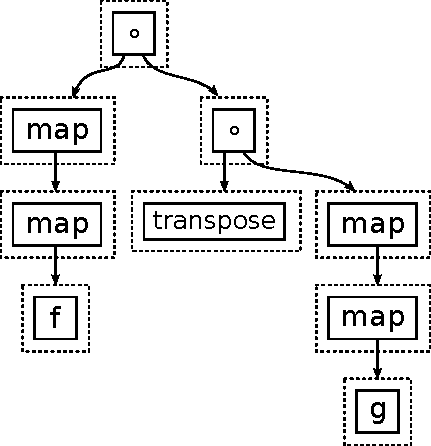
\includegraphics[width=\linewidth]{media/eqsat-example-0.pdf}
  \caption{initialization}
  \label{fig:eqsat-ex-0}
  \end{subfigure}\hfill%
  \begin{subfigure}[b]{0.23\linewidth}
  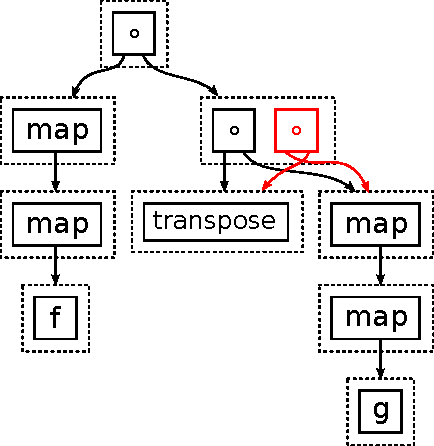
\includegraphics[width=\linewidth]{media/eqsat-example-1.pdf}
  \caption{after rewrite (\ref{overview-move-transpose})}
  \label{fig:eqsat-ex-1}
  \end{subfigure}\hfill%
  \begin{subfigure}[b]{0.23\linewidth}
  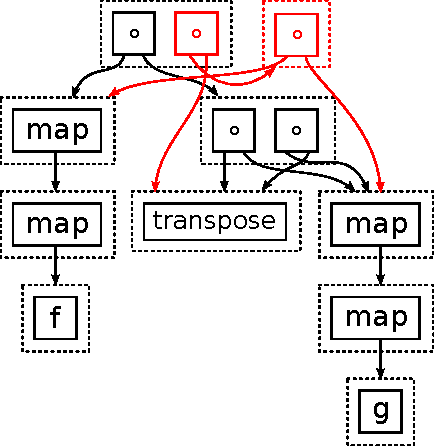
\includegraphics[width=\linewidth]{media/eqsat-example-2.pdf}
  \caption{after rewrite (\ref{overview-comp-assoc})}
  \label{fig:eqsat-ex-2}
  \end{subfigure}\hfill%
  \begin{subfigure}[b]{0.29\linewidth}
  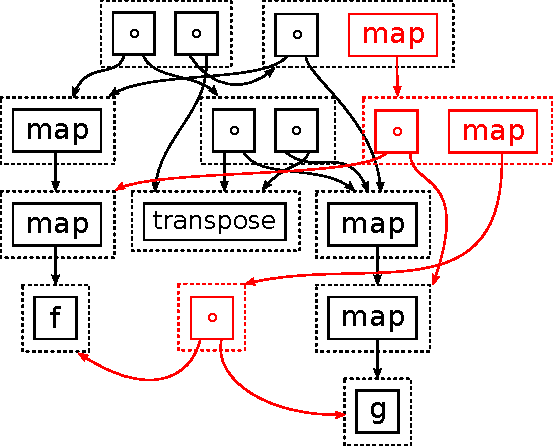
\includegraphics[width=\linewidth]{media/eqsat-example-3.pdf}
  \caption{after two rewrite (\ref{overview-map-fusion})}
  \label{fig:eqsat-ex-3}
  \end{subfigure}
  \caption{Growing an e-graph for the term $(map~(map~f)) \circ (transpose \circ (map~(map~g)))$.
  An e-graph is a set of e-classes themselves containing equivalent e-nodes.
  The dashed boxes are e-classes, and the solid boxes are e-nodes.
  New e-nodes and e-classes are shown in red.}
  \label{fig:eqsat-ex}
\end{figure}
\smallskip

Equality saturation minimizes term size by exploring many rewrites while avoiding local minima.
First, an equality graph (e-graph) representing the initial term is constructed (\cref{fig:eqsat-ex-0}).
An \emph{e-graph} is a set of equivalence classes (e-classes).
An \emph{e-class} is a set of equivalent nodes (e-nodes).
An \emph{e-node} $F(e_1, .., e_n)$ is an $n$-ary function symbol ($F$) from the term language, associated with $n$ child e-classes ($e_i$).
Examples of symbols are $map$, $transpose$, and $\circ$.
The e-graph data structure is used during equality saturation to efficiently represent and rewrite a set of equivalent programs.

The initial e-graph is iteratively grown by applying rules non-destructively (\cref{fig:eqsat-ex-1,fig:eqsat-ex-2,fig:eqsat-ex-3}).
While standard term rewriting picks a single possible rewrite in a depth-first manner, equality saturation explores all possible rewrites in a breadth-first manner.
% independently = "in parallel"
In an equality saturation iteration, rewrites are applied independently: they only depend on rewrites from previous iterations.
% Typically, all possible rewrite rules are applied in every iteration.
For the sake of simplicity, we only apply a handful of rewrite rules in \cref{fig:eqsat-ex}.
When applying a rewrite rule, the equality between its left-hand side and its right-hand side is recorded in the e-graph.
Rewrite rules stop being applied when a fixed point is reached (saturation), or when another stopping criteria is reached (e.g. timeout).
If saturation is reached, it means that all possible rewrites have been explored.

An e-graph represents many equivalent terms and is far more compact than some set of terms as equivalent sub-terms are shared.
E-graphs can represent exponentially many terms in polynomial space, and even infinitely many terms in the presence of cycles \cite{willsey2021-egg}.
To maximize sharing, a \emph{congruence invariant} is maintained: intuitively identical e-nodes should not be in different e-classes (\cref{fig:congruence-invariant}).
Later we will see that even extensive sharing does not necessarily prevent e-graph sizes from exploding.

\begin{figure}
  \begin{minipage}[b]{0.45\linewidth}
    \centering
    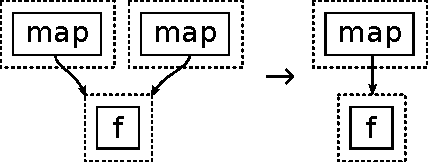
\includegraphics[width=0.6\linewidth]{media/congruence-invariant.pdf}
    \caption{The congruence invariant simplifies the e-graph on the left by merging two identical e-nodes for $map~f$ into a single e-node as shown on the right.}
    \label{fig:congruence-invariant}
  \end{minipage}%
  \hfill
  \begin{minipage}[b]{0.5\linewidth}
    \centering
    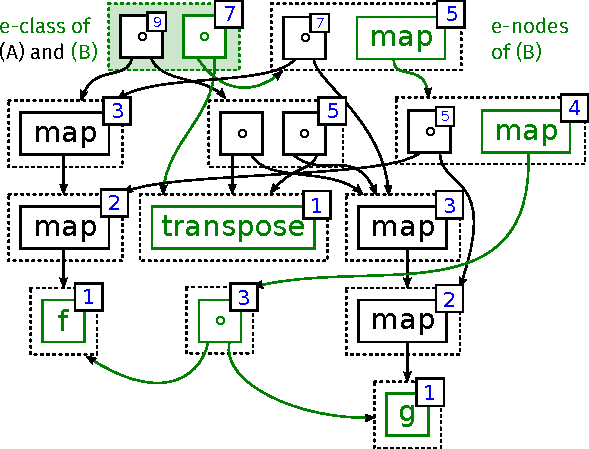
\includegraphics[width=0.8\linewidth]{media/eqsat-example-extract.pdf}
    \caption{Smallest term size computed using an e-class analysis, shown for each e-class in the top-right corner in blue. Where it differs from its e-class value, the smallest term size of e-nodes is also shown. The e-class and e-nodes of the smallest term (\ref{overview-goal}) are shown in green.}
    \label{fig:eqsat-ex-extract}
  \end{minipage}
\end{figure}

After rewriting completes, an \emph{extraction} procedure selects the best term from the e-graph using a cost function. Extraction can use a relatively simple bottom-up e-graph traversal if a \emph{local cost function} $c$  can be defined~\cite{panchekha2015-herbie}. With costs of type $K$, $c$ has signature $c(F(k_1: K, .., k_n: K)) : K$.
More complex cost functions require more complex extraction procedures \cite{wang2020-spores, wu2019-carpentry}.

An \emph{e-class analysis} \cite{willsey2021-egg} propagates analysis data of type $D$ in a bottom-up fashion, and can be used for extraction when the cost function is local.
An e-class analysis is defined by providing two functions: one to $make$ the analysis data from an $n$-ary symbol $F$ combined with the data $d_i$ of its child e-classes; and one to $merge$ the analysis data of e-nodes in the same e-class.
$$ make(F(d_1 : D, .., d_n : D)) : D $$
$$ merge(d_1 : D, d_2 : D) : D $$

To demonstrate e-class analysis, we compute the smallest term in each e-class of our example using an e-class analysis with analysis data $D = (\text{term size}, \text{term})$ as well as $make$ and $merge$ functions below.
The term sizes from the analysis are shown in \cref{fig:eqsat-ex-extract}.
The analysis reveals that there is a smaller term (\ref{overview-goal}) of size 7 in the same e-class as the original term (\ref{overview-start}) which has a size of 9 (top left in \cref{fig:eqsat-ex-extract}).

$$ make(F(d_1, .., d_n)) = (1 + \sum_{i} fst(d_i), F(snd(d_1), .., snd(d_n))) $$
$$ merge(d_1, d_2) = \text{if } fst(d_1) \leq fst(d_2) \text{ then } d_1 \text{ else } d_2 $$

\noindent
% To use the algorithm, the domain of the analysis data together with the $merge$ operation should form a semilattice.

\paragraph{Limitations of automatic rewriting with equality saturation}
In practice, the applicability of equality saturation is limited by scaling issues.
As the e-graph grows, iterations become slower and require more memory.
The growth rate is aggravated by some combinations of rewrite rules, such as associativity and commutativity, that generate an exponential number of equivalent permutations \cite{wang2020-spores, nandi2020-synthesizing-CAD, willsey2021-egg}.
This makes exploring long rewrite sequences inherently hard, as the breadth-first exploration of all possible rewrites leads to an exponential increase of the search space.
We encounter these issues when attempting to optimize matrix multiplication in \Rise{} using equality saturation, as we discuss in \Cref{evaluation}.

Our contributions ameliorate these limitations by minimizing the size of the e-graphs required.
Sketch-guiding factors unfeasible equality saturations into a sequence of smaller, and hence feasible, equality saturations (\cref{sketching}).
Efficient encoding of the $\lambda$ calculus reduces the sizes of the e-graphs produced when optimizing functional programs, like \Rise{} programs (\cref{eqsat-bindings}).